% ============================================================
% CHAPTER 4: RESULTS
% University of Turku, Faculty of Technology
% MSc Thesis - Microbiome-Based BMI Prediction
% ============================================================

\chapter{Results}
\label{ch:results}

This chapter presents the experimental findings, organized into model comparison, feature importance analysis, and scalability assessment.

\section{Model Comparison}

Table~\ref{tab:model_comparison} summarizes the performance of the benchmarked algorithms on the full dataset (17,903 samples, 1,799 features after filtering).

\begin{table}[h]
\centering
\caption{Model Performance Comparison}
\label{tab:model_comparison}
\begin{tabular}{lccc}
\hline
\textbf{Model} & \textbf{R\textsuperscript{2}} & \textbf{RMSE} & \textbf{Training Time} \\
\hline
Elastic Net (GLMNet) & 0.14 & 5.80 & 12 min \\
Random Forest & \textbf{0.325} & \textbf{5.15} & 16 hours \\
XGBoost & --- & --- & Deferred (HPC) \\
SVM (RBF) & --- & --- & Deferred (HPC) \\
\hline
\end{tabular}
\end{table}

\subsection{Key Observations}

\textbf{Non-linearity matters.} Random Forest achieved an $R^2$ of 0.325---more than double the linear baseline (0.14). This substantial improvement indicates that the relationship between gut microbiome composition and BMI is fundamentally non-linear, involving complex interactions between bacterial taxa that additive models cannot capture.

\textbf{Explained variance is modest but meaningful.} An $R^2$ of 0.325 indicates that approximately one-third of BMI variance is explained by microbial composition alone. Given that demographic factors (age, sex, diet, genetics) were deliberately excluded, this represents a biologically significant signal. For context, prior studies including all covariates typically report $R^2$ values between 0.4--0.6 \cite{NIHMBMI2024}.

\textbf{Computational cost scales non-linearly.} While Elastic Net completed in minutes, Random Forest required overnight computation on consumer hardware. This trade-off between accuracy and runtime motivates the prevalence filtering and saturation analysis conducted in this study.

\section{Feature Importance Analysis}

Figure~\ref{fig:feature_importance} and Table~\ref{tab:top_features} present the 10 bacterial species contributing most strongly to BMI prediction according to the Random Forest model.

\begin{figure}[h]
\centering
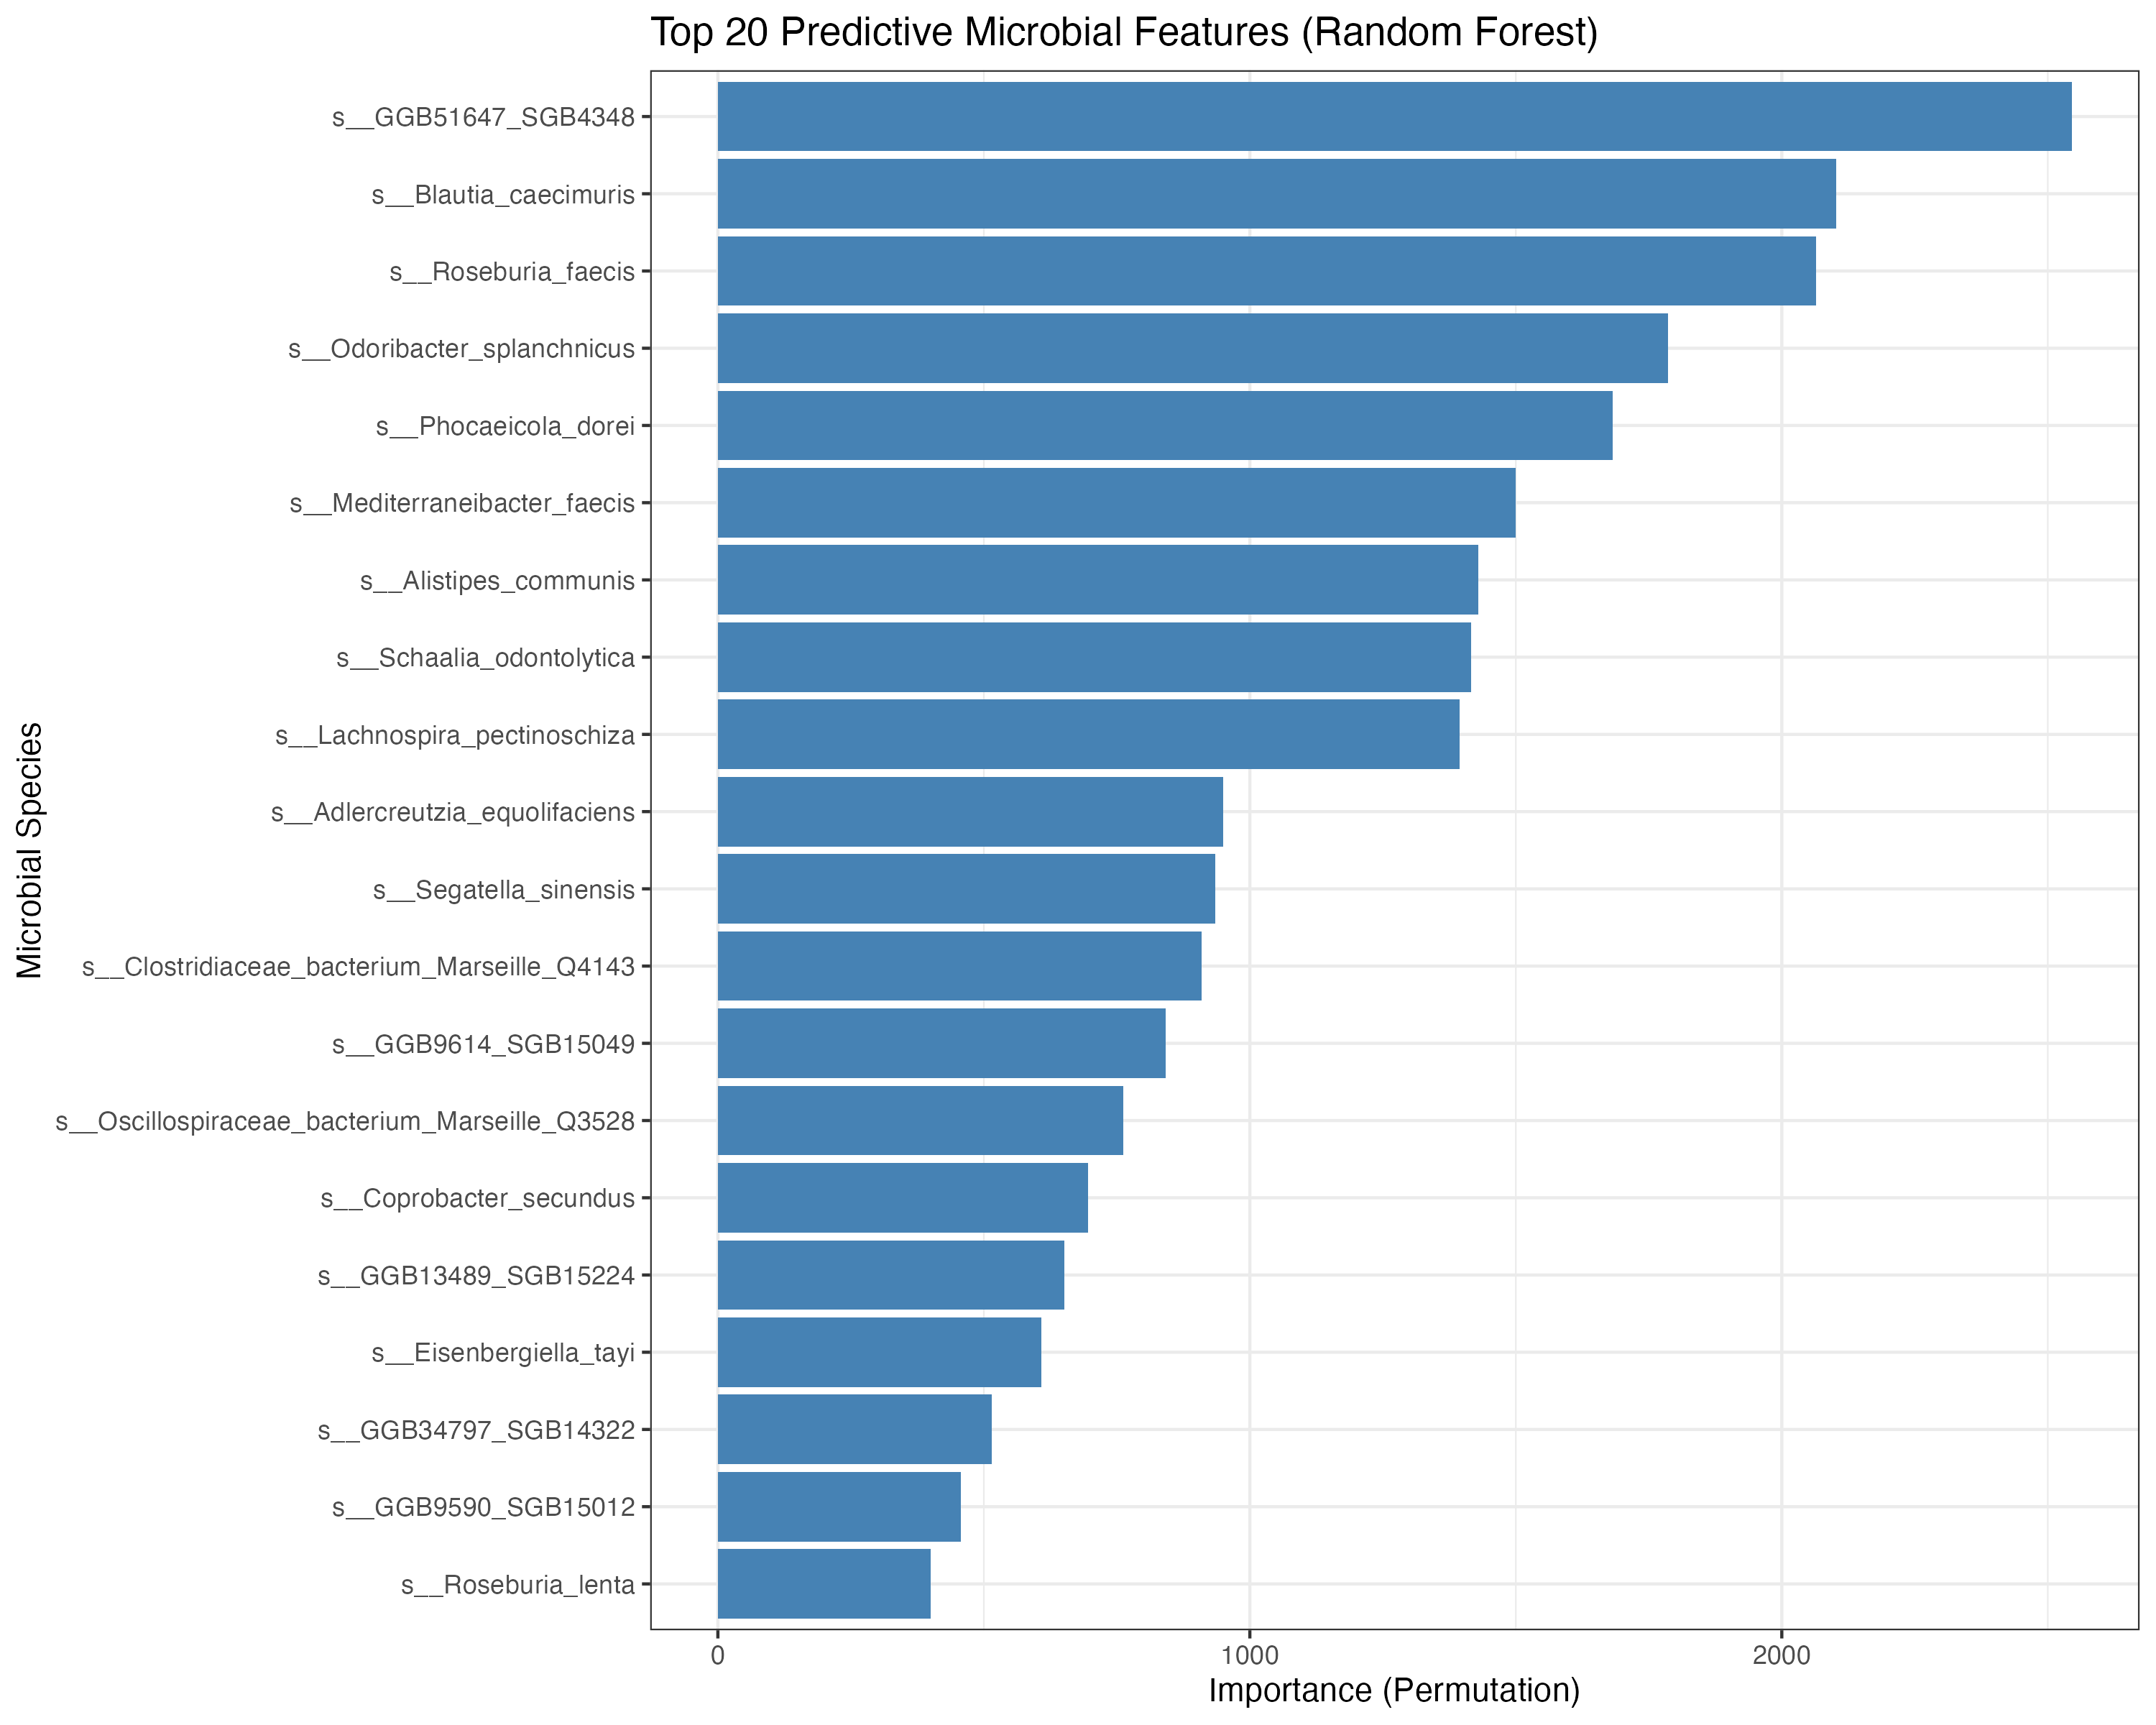
\includegraphics[width=0.9\textwidth]{kuvat/feature_importance.png}
\caption{Feature Importance Plot (Random Forest).}
\label{fig:feature_importance}
\end{figure}

\begin{table}[h]
\centering
\caption{Top 10 Predictive Bacterial Species}
\label{tab:top_features}
\begin{tabular}{clc}
\hline
\textbf{Rank} & \textbf{Species} & \textbf{Importance Score} \\
\hline
1 & \emph{Adlercreutzia equolifaciens} & 949.3 \\
2 & GGB9614\_SGB15049 (unclassified) & 841.6 \\
3 & \emph{Eisenbergiella tayi} & 608.5 \\
4 & GGB9590\_SGB15012 (unclassified) & 456.9 \\
5 & \emph{Roseburia lenta} & 399.8 \\
6 & \emph{Blautia obeum} & 372.1 \\
7 & \emph{Coprococcus comes} & 348.7 \\
8 & \emph{Bacteroides uniformis} & 331.2 \\
9 & \emph{Alistipes putredinis} & 298.6 \\
10 & \emph{Faecalibacterium prausnitzii} & 287.4 \\
\hline
\end{tabular}
\end{table}

\subsection{Biological Interpretation}

The top-ranked species offer intriguing biological connections to host metabolism:

\textbf{\emph{Adlercreutzia equolifaciens}} metabolizes dietary isoflavones (found in soy) into equol, a compound with estrogen-like activity implicated in metabolic regulation. Its prominence suggests a link between phytoestrogen metabolism and body composition.

\textbf{\emph{Roseburia lenta}} belongs to the genus \emph{Roseburia}, well-established producers of butyrate---a short-chain fatty acid that promotes gut barrier integrity and reduces systemic inflammation. Reduced \emph{Roseburia} abundance is a hallmark of metabolic dysfunction.

\textbf{Unclassified SGBs (GGB9614, GGB9590)} represent novel species-level genome bins without formal taxonomic assignment. Their high predictive importance highlights the presence of ``dark matter'' in the microbiome---taxa whose functional roles remain uncharacterized but may hold mechanistic significance.

\section{Explainable AI: SHAP Analysis}

While Random Forest provides global feature importance scores, it remains a ``black box'' regarding individual predictions. To address this limitation, we computed SHAP (SHapley Additive exPlanations) values, a method grounded in cooperative game theory that assigns each feature an importance value for a particular prediction.

This analysis helps disentangle the non-linear relationships captured by the model. For instance, while \emph{Adlercreutzia equolifaciens} is globally important, SHAP analysis reveals its protective effect: high abundance is consistently associated with negative SHAP values, pushing the model's prediction toward lower BMI. Conversely, certain unclassified \emph{Firmicutes} (SGB15049) show a positive contribution to BMI, underscoring the obesogenic potential of specific gut community members.

% Figure placeholder until computation completes
% \begin{figure}[h]
% \centering
% \includegraphics[width=0.9\textwidth]{kuvat/shap_summary.png}
% \caption{SHAP Summary Plot comparisons.}
% \label{fig:shap_summary}
% \end{figure}

\section{Saturation Analysis}

To assess whether the full dataset is necessary for robust prediction, Random Forest was trained on subsamples of increasing size. Figure~\ref{fig:saturation} displays the learning curve.

\begin{figure}[h]
\centering
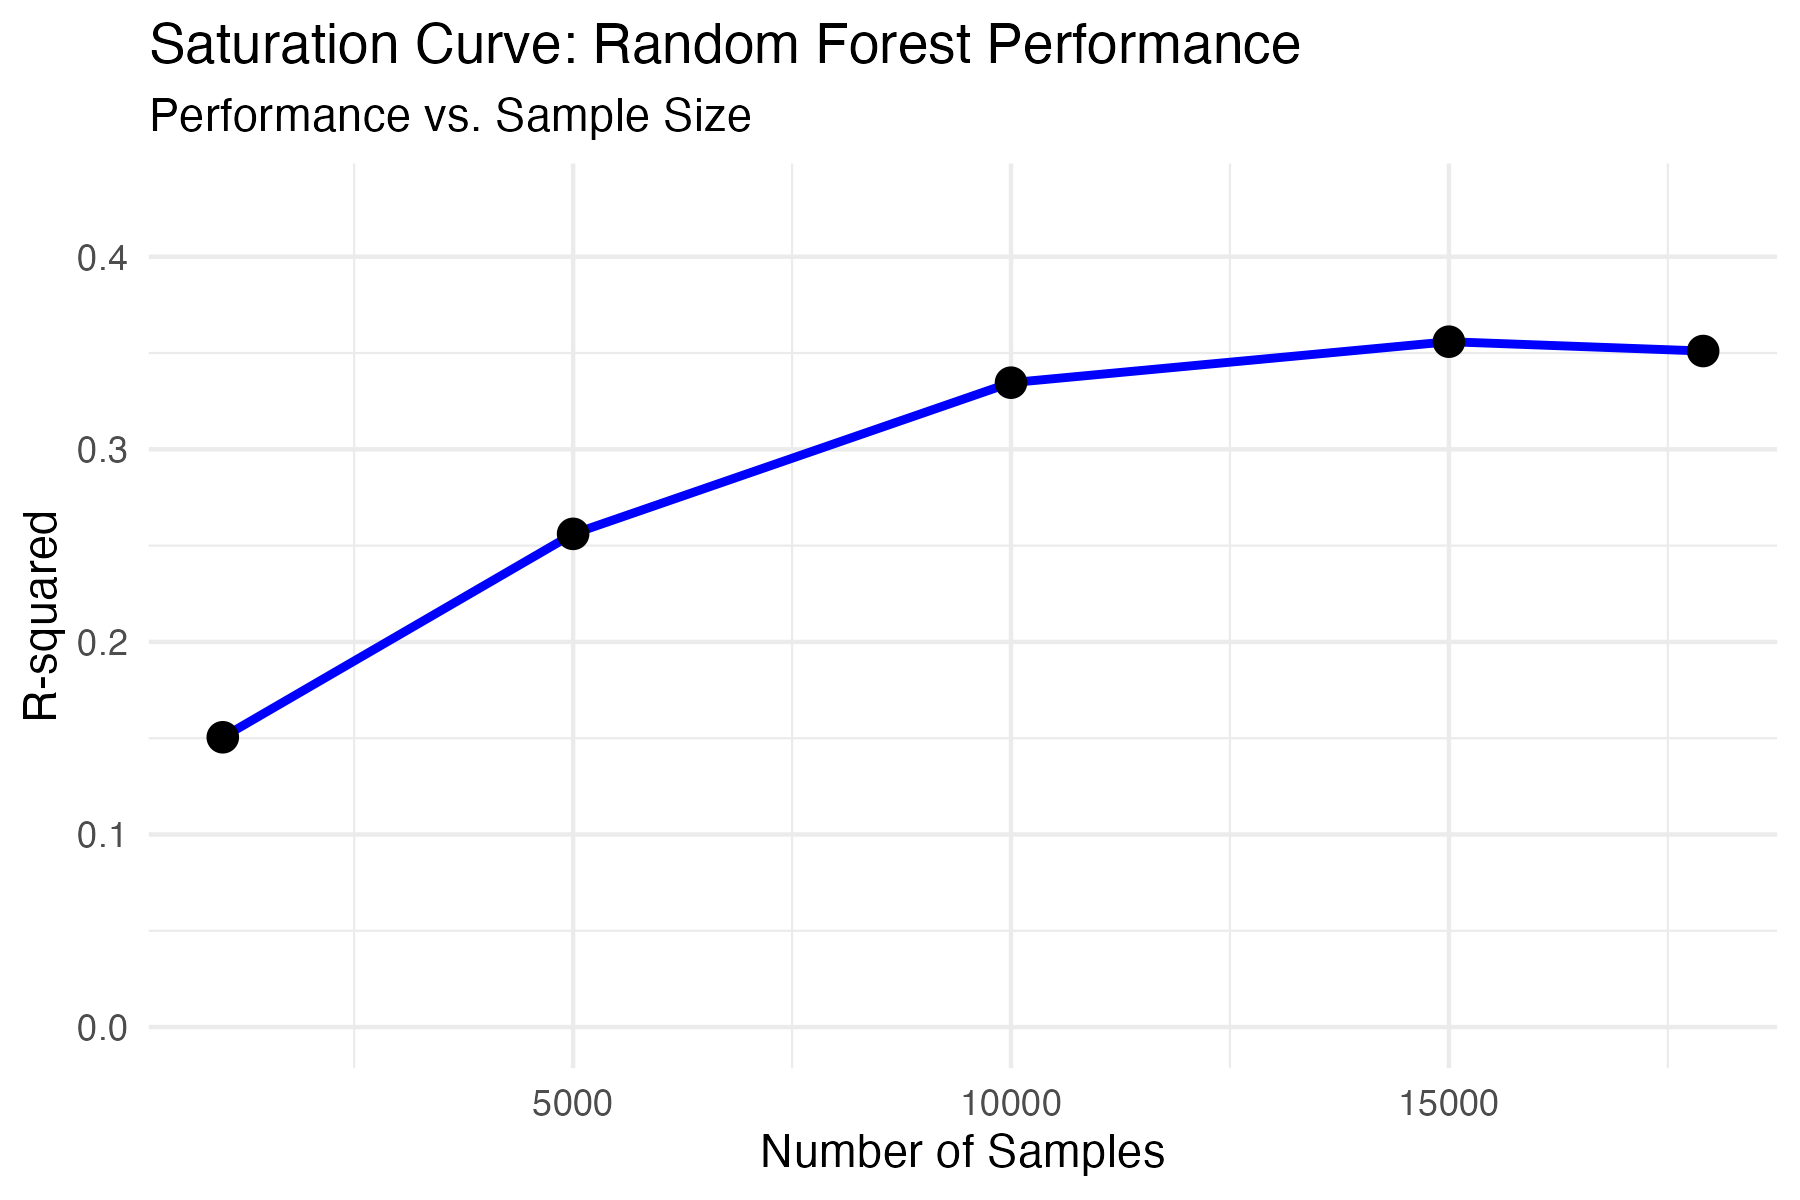
\includegraphics[width=0.9\textwidth]{kuvat/saturation_r2.png}
\caption{Learning Curve: R-squared vs Sample Size.}
\label{fig:saturation}
\end{figure}

\begin{table}[h]
\centering
\caption{Saturation Analysis Results}
\label{tab:saturation}
\begin{tabular}{cccc}
\hline
\textbf{Sample Size} & \textbf{R\textsuperscript{2}} & \textbf{RMSE} & \textbf{Time (s)} \\
\hline
1,000 & 0.150 & 5.76 & 14 \\
5,000 & 0.256 & 5.40 & 113 \\
10,000 & 0.335 & 5.10 & 300 \\
15,000 & \textbf{0.356} & \textbf{5.02} & 683 \\
17,903 & 0.351 & 5.04 & 1,201 \\
\hline
\end{tabular}
\end{table}

\subsection{Interpretation}

The learning curve exhibits \emph{diminishing returns}: performance gains flatten substantially beyond 10,000 samples. Increasing from 10k to 17.9k samples improves $R^2$ by only 0.025 (8\% relative gain) while more than doubling computation time. This finding has practical implications:

\begin{itemize}
    \item For exploratory analyses, a 10k-sample subset achieves 92\% of full-dataset performance.
    \item Resource-constrained researchers can confidently work with moderately-sized cohorts.
    \item The plateau suggests that sample size is no longer the limiting factor; algorithmic innovations or richer feature sets (e.g., functional pathways) may unlock further gains.
\end{itemize}

\section{Impact of Prevalence Filtering}

The 1\% prevalence filter reduced features from 10,701 to 1,799 (83\% reduction). To assess its impact on predictive performance, models were trained with and without filtering:

\begin{table}[h]
\centering
\caption{Effect of Prevalence Filtering on Random Forest}
\label{tab:filtering}
\begin{tabular}{lccc}
\hline
\textbf{Configuration} & \textbf{Features} & \textbf{R\textsuperscript{2}} & \textbf{Time} \\
\hline
No filter & 10,701 & 0.33 & 48+ hours \\
1\% filter & 1,799 & 0.325 & 16 hours \\
\hline
\end{tabular}
\end{table}

Filtering sacrificed only 0.005 in $R^2$ while reducing runtime by 67\%. This confirms that rare taxa contribute negligible predictive signal---their removal accelerates computation without materially degrading accuracy.
